\documentclass[../main/main.tex]{subfiles}
\begin{document}

\chapter{Engineering.}

\section{Cooling systems.}

I was prompted by \href{https://www.youtube.com/watch?v=9CodKUa4F2o}
{this YouTube video}
(which discusses \href{https://www.ncbi.nlm.nih.gov/pmc/articles/PMC3062901/}
{this 2002 paper})
and a discussion I had with my housemates when trying
to diagnose why our central air conditioning system
working \textemdash{}
how \emph{do} cooling systems work?
Systems naturally \emph{produce} heat during operation,
not ``consume'' it from its surroundings\footnote{
    Though how amazing (and law-breaking)
    would it be if we were to find a machine that
    could consume more heat energy than it produces!
    \href{https://en.wikipedia.org/wiki/Perpetual_motion\#Basic_principles}
    {I wouldn't hold my breath for that though.}
}, so operating any ol' system should \emph{increase}
the nearby temperature, not decrease it.
Now, the explanation for how a cooling system works
usually goes something along the lines of
``\textit{something something} refrigerant 
\textit{something something} condenser pipes
\textit{something something} cooler air.''
But how does the refrigerant absorb the heat,
how does it later release the heat,
how does it circulate in the first place,
how do the condenser pipes actually condense, etc etc.?
(None of these are necessarily difficult questions to answer
\textemdash{} I just rarely seem them addressed.)

\subsection{An overview.}

We shall give a broad overview of what happens, deferring
(practical and important questions) after the general
flow of action is laid out.\par

(Hot) air enters from inlet ducts 
and passes \emph{across}
the actual cooling loop, a closed system where \emph{refrigerant}
flows cyclically (ala a pump).
The cooling loop absorbs energy from the air as the air passes 
across the system. A fan meets the cooled air at the other end
of the cooling loop, where it pushes the air through outlet ducts
to allow the attached room to enjoy cooler temperatures
(and drier air).

\subsection{Questions and answers.}

The overview was pretty vague and ought to raise a number of questions.
Let's go through them.

\subsubsection{What's a refrigerant?}

A \textbf{refrigerant} (or \textbf{coolant}) is a chemical whose
properties make it useful in this heat-siphoning loop we're trying
to make. So what exactly are the properties we're looking for?\par

Conventional cooling systems rely on the \textbf{enthalpy of fusion}
(and conversely, the \textbf{enthalpy of evaporation}),
a measure for the change of free energy of a substance when it undergoes
a \emph{phase transition} from gas to liquid
(and conversely, from liquid to gas).
As a general rule, energy must be put into a substance in order to change
it from its liquid state to its gas state, and energy must be removed
from the substance for it to condense back down to its liquid state.
The energy can be applied or extracted in a few different ways. 
The most relevant ways will be from 
\begin{enumerate}
    \item
    \emph{heat flow} into or out of a system
    (a spontaneous flow of energy due to a temperature difference between the
    system and its surroundings in the direction which tends toward
    thermal equilibrium \textemdash{} a universal observation codified
    by the second law of thermodynamics\footnote
    {
        Technically, the thermodynamics rule dictates spontaneous flow of energy
        in order to increase the overall \emph{entropy} of the universe.
        Outside of extremely pathological cases though,
        approaching thermal equilibrium \emph{does} increase the overall entropy
        of the universe, and so saying it's due to a ``temperature difference''
    }); or from 
    \item
    \emph{work done} to a system or by a system
    (where \emph{work} is used in the physics sense and implies force-distance
    or pressure-volume work).
\end{enumerate}

\subsubsection{Better specifying ``heat'' and our problem.}

It's worth noting the ambiguity that comes from 
``heat'' in the thermodynamics sense and ``heat''
in more colloquial senses.
\begin{enumerate}
    \item
    Thermodynamic ``heat'' refers specifically to the phenomenon of energy
    transfer due to temperature difference between systems.
    That is the meaning of heat used in our list of methods of energy transfer.
    So \emph{no system ``contains'' heat in the thermodynamic sense}.
    \item 
    A more colloquial use of ``heat'' as the thing we're trying to remove
    via a cooling system is more closely related to the \emph{internal energy}
    (or relatedly, due to Legendre transformation, the enthalpy)
    of a system. The internal energy \emph{is} a quantity that a system
    can be said to ``have'' and is strongly associated with the temperature
    of the system.\footnote
    {
        In fact, for the simple case of a system comprised solely of an ideal gas,
        a system's internal energy can be exactly equal to its kinetic energy,
        which, for an ideal gas, is directly proportional to its temperature.
    }
    \item
    There's also the use of ``heat'' as describing the wasted energy by a
    process that is not 100\% efficient.\footnote
    {
        Read: literally every process
        known to humanity at this point. We're
        lucky if we push past something like 
        30\% efficiency.
        Even the method by which our bodies extract
        energy from food is
        \href{http://history.cpet.ufl.edu/lm/respiration/efficiency01.html}
        {just under 40\% efficient} (and that's
        \emph{incredibly} good).
    }. This meaning is often used in a phrase
    like ``[some energy] is \emph{given off} as heat'' or
    ``the rest [of the energy] is \emph{lost} as heat''.
    The word \emph{lost} is used because this wasted energy cannot be
    immediately harnessed to perform (pressure-volume, force-distance, etc.)
    work. This use of heat actually also ties into the \emph{internal energy}
    meaning, as this heat increases the \emph{kinetic energy of the molecules
    in the surroundings} (and this microscopic kinetic energy counts as
    part of the internal energy of the surroundings).
\end{enumerate}
We shall continue forward by using \emph{heat} to refer to the phenomenon
of energy transfer and \emph{internal energy} or \emph{thermal energy}
to refer to the property
related to the energy of the system in question. We shall probably
also say that some energy ``is lost as heat'', where we'll mean
heat in the ``wasted''-energy sense.\par

OK, so what exactly is the goal of a cooling system then?
Say the air conditioning system is servicing a house. Then the immediate
goal is to remove internal energy from (and so lower the temperature of)
the air in the house.
But at the same time, we want to remove the internal energy from the entire
air-house-coolant system (by dumping said energy out via an exhaust)
to have a cooling cycle that is ``sustainable'' for when the air
inevitably warms up from the air-house-coolant system being in contact
with a warmer set of surroundings.
Both of these conditions need to be met to have a cooling system
that works and can work more than one time.
% remove internal energy (and so lower the temperature) of air+house+coolant system
% (dumping out the energy through an exhaust outside the system)

\subsubsection*{OK, but you never explained what properties a refrigerant
should have.}
You're right; let's do that now.\par

We were talking about enthalpies of evaporation and fusion earlier.
The former shall be our ``sponge'' with which we'll absorb energy
from the hot air (thus making it cooler),
and the latter will be how we wring out our sponge 
in order to have it absorb more energy.
Appropriately, the pipes that cause the refrigerant to
evaporate and condense (``fuse'') are called
\emph{evaporator pipes} and \emph{condenser pipes}.
In fact, they're both \emph{coils} of pipe \textemdash{}
this improves space efficiency and increases the surface area
through which the refrigerant can absorb energy from the air
(in the evaporator coils) or release energy to prepare for
the next cycle (in the condenser coils).\footnote
{
    Increasing surface area relative to volume is a common
    tactic in increasing the ``flow'' of some quantity
    into or out of a system. For a biological example,
    consider the villi and microvilli in the human intestine. 
    These features increase intestinal surface area
    by over an order of magnitude and consequently greatly
    increase our ability to absorb nutrients from the food
    we eat.
}\par

Now, it would be kind of silly to use a ton of energy
to either cool down or heat up our refrigerant to get to
somewhere near its phase-transition temperature.
Why put in all that (literal and metaphorical) work when
there are compounds that naturally have boiling points near
room temperature?
And that's really the main property we're looking for in
a refrigerant: we wants its boiling point to be no more
than a dozen or so degrees centigrade
from the desired room temperature (often near 20 \textdegree C),
perhaps with an even smaller differential if the
refrigerant has a large \emph{heat capacity}.\footnote
{
    In general, we'd want the refrigerant to have a high enough
    heat capacity and boiling point so that it will evaporate
    after absorbing a large enough ``heat load'' from the house air
    so that the house air actually decreases in temperature
    a significant amount \textemdash{} if it only takes ten joules
    to evaporate all your refrigerant, it's going to take a lot
    of time and externally applied energy to cool the room
    (if the rate of heat efflux would even counteract the
    rate of heat influx).
} The 
\emph{viscosity} of the substance in the liquid form is
also important \textemdash{} we're going to have to pump this
thing repeatedly, so it'd be nice if it doesn't stick to the walls
like an ``overdeveloped'' squeeze-bottle of honey.\par

As a practical note, it wouldn't make sense to wring out our sponge
\emph{inside} our house, as that would simply return the heat
back into the air we're trying to cool.
So condenser coils ought to be located near an outlet of
the air-house-coolant system so that we can ``dump'' the excess
energy outside via, say, an exhaust fan.
Now when the refrigerant condenses, the condenser pipes warm up
and eventually radiate out the excess energy into the surroundings.
% So a refrigerant would change phase near room temperature, so that
% we can have it change phase "easily" and without needing to use up energy
% just to keep the refrigerant near its phase-transition temperature

\subsection{How do we push things along? Pumps and valves.}

Now that we've determined what sort of substance we want to use,
we need to cyclically push this substance along our cooling circuit.
How?
Pumps and valves powered by good ol' electromechanical energy.
(The need for external power and subsequent increased
electric bill is why you probably 
don't always leave your house
at a crisp 20 \textdegree C).
Right before the compressor pipes is a \emph{compressor valve}
which holds the refrigerant and pumps it into the condenser pipes
as appropriate (via an internal thermostat, barometer,
etc. \textemdash{} we don't want to blow any pipes!).
By pushing the refrigerant into the condenser pipes, the refrigerant
gets pressurized and condenses as a result. Why does it undergo
increased pressure?
\emph{The condenser pipes
\textbf{have a smaller cross-sectional area}
than previous pipes},
and so forcing the refrigerant into these narrower tubes 
increases the pressure on and density of the refrigerant.
Then bam, condensation! And subsequent release of internal energy.
% How phase change? Condensor pipes literally just get thinner, 
% and with valves and pumping motion, pushes the gas molecules 
% close enough to condense

% How would valves/pumps work? Forcibly via converting electricity to mechanical work


\subsubsection{Short tangent on biological valves.}
% TODO: Could use a figure demonstrating the
% ``flappiness'' and orientation of the valves.
At some point during this rabbit hole, I realized that what
works for electromechanical valves does not translate to (at least most)
valves in the human body, particularly the valves along our veins.
How do \emph{these} valves work to prevent backflow of blood?
Are we constantly sending electrical stimuli to all the veins' valves
in tandem with diastole in order to prevent backflow?\par

Turns out, it's much simpler than that. (See Fig. \ref{fig:vein-valve-function}.)

\begin{figure}
\centering
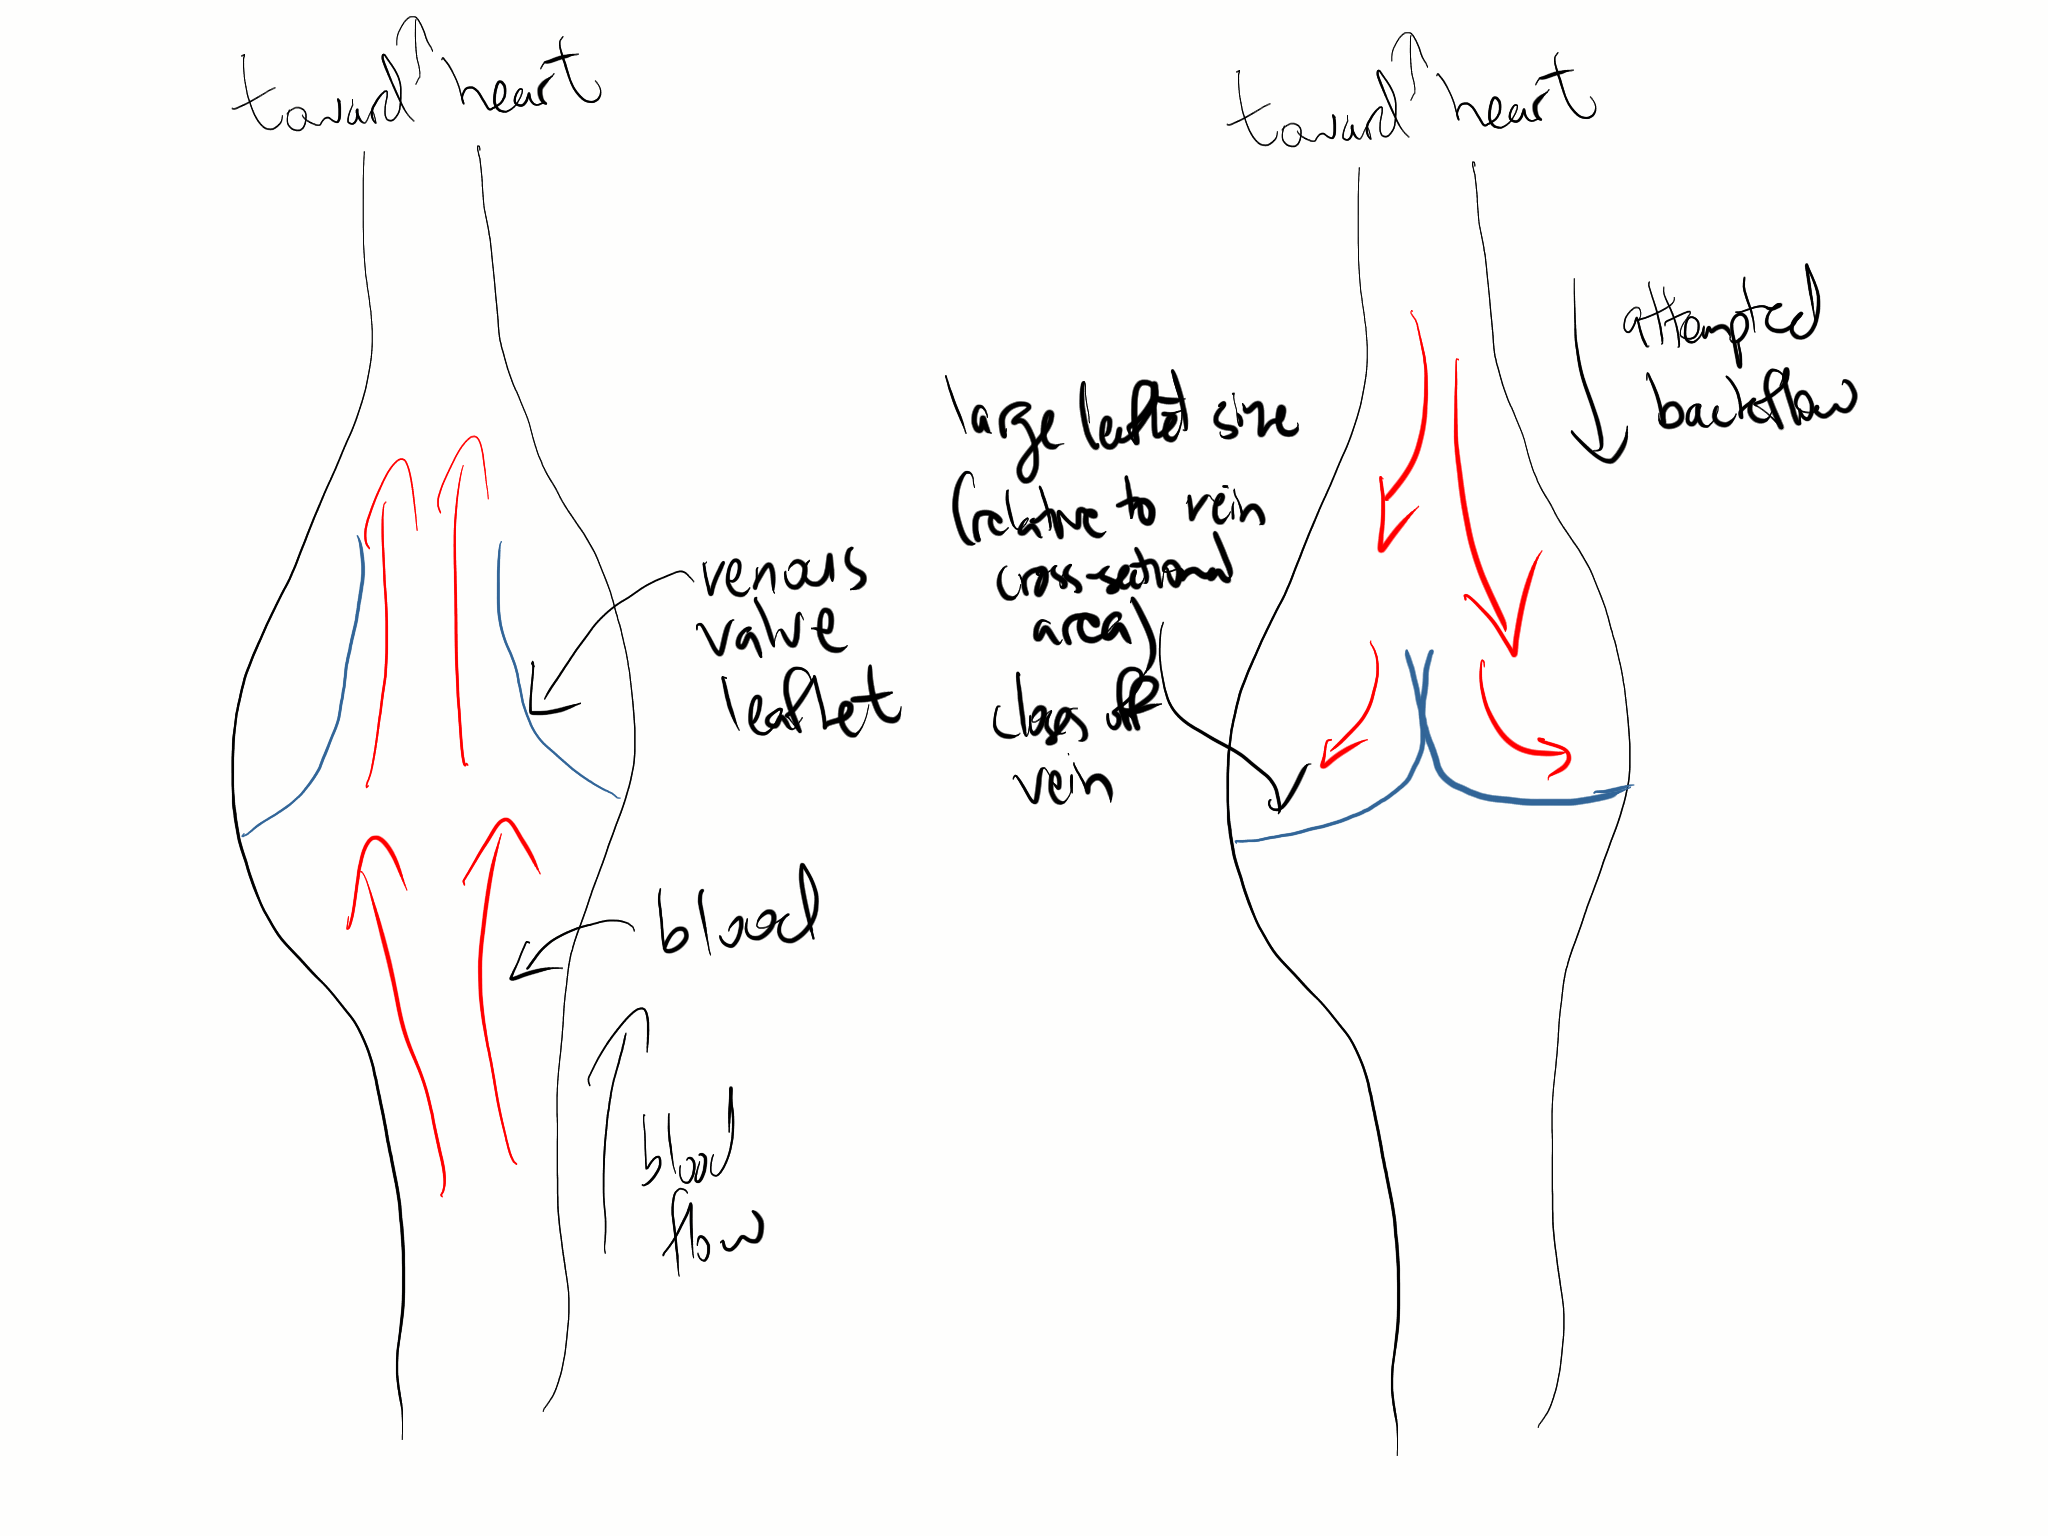
\includegraphics[width=1.0\linewidth]{../img/engineering/vein_valve_function.png}
\caption{
\textbf{Cartoon of normal venous valve function.}
The ``excess'' size of the leaflets which comprise
the vein's valve prevent blood backflow.
% (Image taken from \href{https://www.varicoseveindr.com/images/NORMAL-AND-ABNORMAL-VALVE.jpg}{here} (and apparently originally from
% a text on sclerotherapy published by Elsevier
% in 2007).)
}
\label{fig:vein-valve-function}
\end{figure}

The venous part of our circulatory
system is parallel to the earth's gravitational field when we're
standing, and the pumping action of the heart pushes the blood
against said gravitational field. So we just need some way
to prevent blood from ``falling down''.
Well, let's make our valve out of flaps that are too ``big''
from the circular area of the vein itself, and let's
have the ``excess'' portion of the flaps point upward.
Now, as blood rushes ``forward''
toward the right atrium of the heart,
there is much less ``friction'' provided by the flaps
of the valve \textemdash{} the rushing blood can
push the flaps aside.
But if blood moves \emph{backward}, it necessarily
would have to pull the flaps of the vein's valve along
with it. And since the flaps are too big, they aren't easily
pulled past each other to start facing down
(i.e., they can't easily undergo \emph{prolapse})
and so they instead shut closed. So the blood's ``attempt''
at backflow itself (naturally caused by
gravity's pull) causes the venous valves to close,
thus preventing backflow.
So our circulatory system uses gravitational pull
and the blood itself in order to prevent backflow of blood
in the veins. I'd say that's pretty darn neat!

\subsection{What facilitates heat transfer from the air to the refrigerant?}

Something that may be obvious is that the house's air and the refrigerant
never come into direct contact with one another.
They're always separated by the pipes which house the refrigerant.
So what allows for heat transfer from air to refrigerant?
The pipes! On the evaporator side of things, the pipes get warmed up
externally by the hot air. The material of the pipe then ``spreads out''
the internal energy gained by the hot air, since spreading it out
increases the entropy of the system comprised by the pipe.
So now both ends of the pipe's wall, as well as the thickness of the wall,
``hold'' some amount of the internal energy bestowed upon it by the hot air.
But the pipe is also in contact with a cooler material (the refrigerant),
so in service of reaching thermal equilibrium, there is heat transfer
to the refrigerant from the pipe's interior wall (their contact point).
In this way, the pipe mediates heat transfer between house air and refrigerant.
You can imagine that something similar happens and the condenser side of things,
except that now the warmer body is the refrigerant/pipe interior
and the cooler body is the outside air, and so thermal equilibrium dictates
heat transfer from the refrigerant to the outside air.

\subsection{Conclusion.}

...And I think those are the questions that I kept having about
air conditioner function.
It's worth noting that the system described above can be used
to either cool \emph{or} heat a room. To do the latter,
you literally just have the refrigerant go through the cycle
in the opposite direction, where now the refrigerant evaporates
from internal energy from the outside and condenses in the coils
on the inside, giving off energy to increase the temperature
inside. Cooling systems that can perform these two functions
(and necessarily ventilation, because otherwise how are you
going to move air into or out of the house/building?)
are called \textbf{HVAC systems},
where HVAC stands for 
``heating, ventilation, and air conditioning''.\par

It's interesting to note a similar notion of
``pass coolant through a tube''
can be used in other contexts.
Liquid cooling systems use water and its high heat capacity
(contained in a tube, of course!)
to absorb energy from the high-temperature surroundings of the
CPU of a computer, server, or other device in high load, where
temperatures can reach in excess of 100 \textdegree C.
\href{https://auto.howstuffworks.com/cooling-system.htm/printable}
{The cooling system of a car} also involves passing
fluid past hotter places to have them cool down, then having
the fluid release the energy into the nearby air.
In these cases, the coolant does not undergo a phase transition.
It actually doesn't \emph{need to}, because just by
the tendency toward thermal equilibrium and by 
having fluid with an appropriate heat capacity,
these cooling methods
will always have heat flow from higher-temperature systems
to lower-temperature systems.\footnote
{
    I presume this method
allows for (faster) cooling with larger absolute differences
in temperature between system and surroundings 
(because the coolant can handle larger thermal loads) but
requires more energy per cycle than a phase change-based
temperature control method, especially across large 
distances
(and \emph{especially} large \emph{vertical} distances).
It's generally much easier to pump a gas than a liquid due
to the former's lower density. If the entire system
that need's to be cooled is only within a few feet
from each other, sure, pumping liquid isn't that big a deal
compared to the gains in thermal load we can achieve
by giving our coolant a much wider region in phase space
it can occupy.
But try pumping a liquid up a skyscraper and you should
quickly see why such a method is not viable to use the
same method to cool down buildings!
}\par

It's amazing how a seemingly simple desire to cool something
down requires quite a bit of knowledge of chemistry, physics,
material science, and thermodynamics in order to formulate
a working solution, and how different flavors of that solution
allow for the operation of machines that are critical in
the everyday function of today's society.
(And this is hardly the only such critically
important solution!)
\\
\\
- DK, 7/18/18

\end{document}